
\documentclass[xcolor=pdftex,table,11pt]{beamer}
\usetheme{Warsaw}
\usepackage[utf8]{inputenc}
\usepackage[spanish]{babel} 
\usepackage{amsmath}
\usepackage{amsfonts}
\usepackage{amssymb}
\usepackage{multirow}
\usepackage{siunitx}
\usepackage{listings}
\usepackage{tabulary}
\usepackage[highlightcolor=yellow]{../styles/code}
\author{Informática I\newline Centro Regional Universitario Córdoba\newline UNDEF }
\title{Clase II: \newline Etapas de un programa en C  \newline  Buenas prácticas de programación  \newline Estructura switch}
\setbeamertemplate{footline}{}
\usepackage{booktabs}
\usepackage{longtable}
\newcommand*{\thead}[1]{\multicolumn{1}{c}{\bfseries #1}}


%\setbeamercovered{transparent} 
%\setbeamertemplate{navigation symbols}{} 
%\logo{} 
%\institute{} 
%\date{} 
%\subject{} 
\begin{document}


\begin{frame}
\titlepage
\end{frame}

\begin{frame}{Etapas de un programa en C }

 \begin{enumerate}
   
     	\item<1->  Escritura del código fuente: se pueden utilizar diferentes editores de texto: gedit, VIM, Zinjal, Atom, Emacs, etc. 
     	
\href{https://github.com/danis963/informaticaI_IUA/blob/main/c/c_detras_de_escena/volumen_esfera.c}{\beamergotobutton{Ver en github}}


        \item<2->  Pre-procesamiento: procesa directivas como $\#$include, $\#$define e $\#$if, remueve los comentarios, etc. En general, luego del preprocesamiento, el archivo resultante contiene una gran cantidad de líneas de código.
       
		\href{https://github.com/danis963/informaticaI_IUA/blob/main/c/c_detras_de_escena/volumen_esfera.i}{\beamergotobutton{Ver en github}}
		
		
	\item<3->  Compilado: el compilador de C traduce el código del apartado anterior a assembler. 
     
		\href{https://github.com/danis963/informaticaI_IUA/blob/main/c/c_detras_de_escena/volumen_esfera.s}{\beamergotobutton{Ver en github}}
		
		
				\item<4->  Ensamblado: el ensamblado transforma el programa escrito en lenguaje ensamblador a código objeto. 
		
		\href{https://github.com/danis963/informaticaI_IUA/blob/main/c/c_detras_de_escena/volumen_esfera.o}{\beamergotobutton{Ver en github}}

				\item<5->  Enlazado: reune uno o más módulos en código objeto con el código existente en las bibliotecas.
		
		\href{https://github.com/danis963/informaticaI_IUA/blob/main/c/c_detras_de_escena/a.out}{\beamergotobutton{Ver en github}}

   \end{enumerate}

\end{frame}
   \begin{frame}
   \begin{figure}

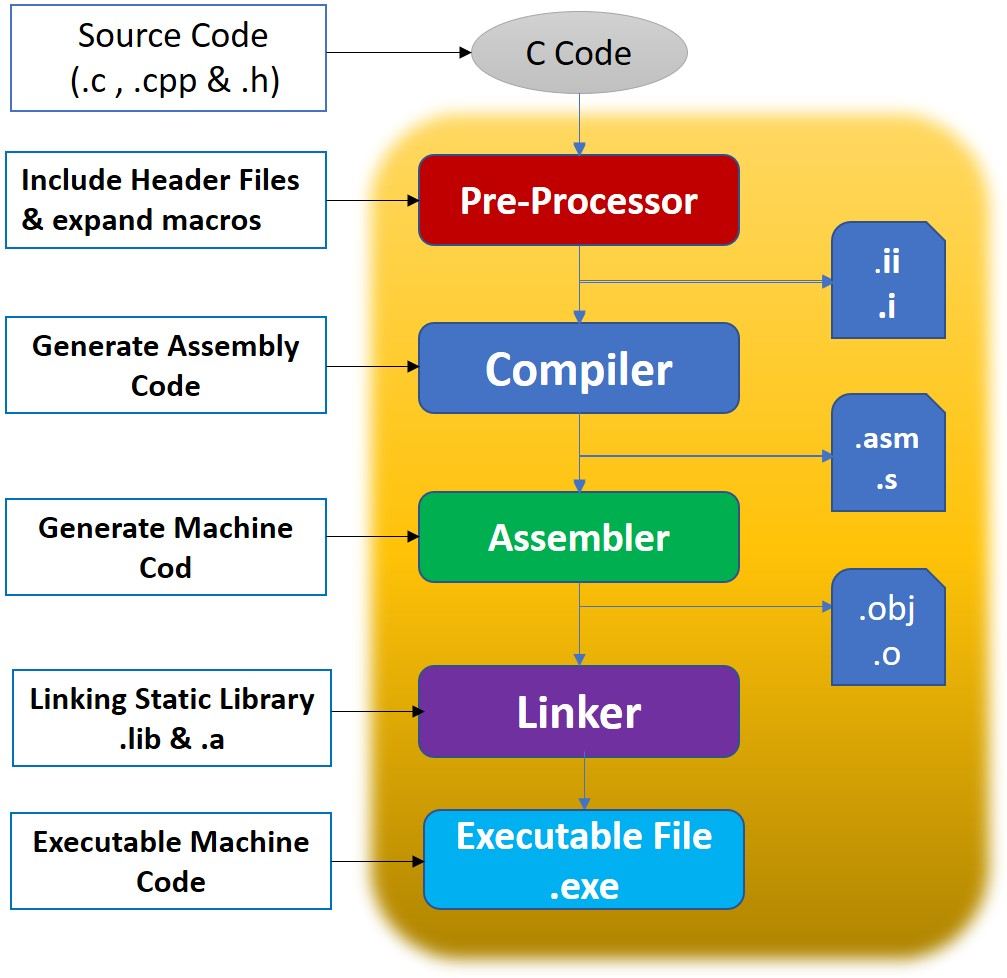
\includegraphics[scale=0.35]{../img/exported/c_step_processes.jpg}
\caption{Etapas de un programa en C.}
\end{figure}
Estos ejemplos fueron generados agregando el flag "-save-temps" al compilador gcc. 


\end{frame}




\begin{frame}{Buenas practicas de programación}
\begin{itemize}

\item<1-> Proyectos con aproximadamente 300.000 lineas de código o menos
\begin{itemize}
\item<1->  Aplicación promedio para smartphone
\item<2->  Photoshop v1.0 (1990)
\item<3->  Quake 3 (1999)
\item<4->  Transbordador espacial STS (1981)
\end{itemize}

\item<5-> Proyectos con aproximadamente menos de 10 millones de líneas de código
\begin{itemize}
\item<6->  Age of empires - Versión online
\item<7->  Linux kernel 2.2.0
\item<8->  Windows 3.1 (1992)
\end{itemize}


\item<9-> Proyectos con aproximadamente más de 50 millones
\begin{itemize}
\item<10->  Age of empires - Versión online
\item<11->  Linux kernel 2.2.0
\item<12->  Windows 3.1 (1992)
\end{itemize}



\item<13-> Proyectos con aproximadamente más de 2 mil millones de líneas de código
\begin{itemize}
\item<14->  Google Internet Services
\end{itemize}


\end{itemize}



\end{frame}



\begin{frame}{Buenas practicas de programación: reglas de estilo}
\begin{itemize}
\item<1-> Variables 
	\begin{itemize}
		\item<2-> Los nombres deben ser cortos, descriptivos y concretos
		\item<3-> Si el nombre contiene dos o más palabras, se las debe separar por \_
		\item<4-> Deben inicializarse a un valor conocido al momento de la declaración
	\end{itemize}
	
\item<5-> Constantes definidas con \# define 
	\begin{itemize}
		\item<6-> Su identificador debe escribirse con mayúsculas
	\end{itemize}



\item<7-> Indentación del código
	\begin{itemize}
		\item<8-> Debe realizarse con tabulaciones, nunca con espacios
		\item<9-> Deben colocarse llaves para demarcar gráficamente el código que ejecutará cada estructura

		\item<10-> Las llaves deben escribirse siempre
		
		\item<11-> Las líneas de código no deben superar la longitud de 80 caracteres

		
	\end{itemize}

\item<12-> Instrucciones que se deben evitar
	\begin{itemize}
		\item<13-> goto
		\item<14-> Break
		\item<15-> Continue

		
	\end{itemize}

\end{itemize}

    
\end{frame}


\begin{frame}{Estructura Switch}

 \begin{block}{Aplicación}
 Permite que un programa en C tome diferentes caminos en función del valor que tome una determinada instrucción.
 
 
 \end{block}

 \begin{block}{Pseudocódigo}

    \begin{itemize}
   \item[]Según sea (variable de control)
   \begin{itemize}

     	\item[] Caso 1:
     	    \begin{itemize}
     			\item[] Instrucciones caso 1
     			\item[] Instrucciones caso 1
     			\item[] frenar
     		   \end{itemize}

        \item[] Caso 2:
     	    \begin{itemize}
     			\item[] Instrucciones caso 2
     			\item[] Instrucciones caso 2

     			\item[] frenar
 		
   			\end{itemize}
    
    \item[] Caso por descarte
     	    \begin{itemize}
     			\item[] Instrucciones caso por descarte
     			\item[] frenar
 		
   			\end{itemize}

   \end{itemize}

	\end{itemize}

 \end{block}

\end{frame}



\begin{frame}{Estructura Switch}

\begin{figure}

\includegraphics[scale=0.201]{../img/exported/switch.png}
\caption{Diagrama de flujo para la estructura switch}
\end{figure}
\end{frame}


\begin{frame}{Estructura Switch}
\codesetstylefrombeamer
\cppfile{../../c/src/1-2_switch_case.c}
\end{frame}


\begin{frame}[allowframebreaks]{Estructura Switch - ejemplos}
 \begin{enumerate}
   \item Diseñar y codificar un programa que permita tomar por teclado un número entero comprendido entre 0 y 2 inclusive. Luego el programa imprimir por pantalla la opción seleccionada en modo texto. Si el usuario ingresa una opción invalida, debe informarse dicha excepción por pantalla.
      \href{https://github.com/danis963/informaticaI_IUA/blob/main/c/src/1-2_switch_case.c}{\beamergotobutton{Ver en github}}
           
       \item Diseñar y codificar un programa que permita tomar por teclado un número entero. Este número entero representa un mes del año, siendo 1 para enero y 12 para diciembre. El programa debe imprimir por pantalla la cantidad de días del mes seleccionado. \footnote{Se supone un año no bisiesto.}
       \href{https://github.com/danis963/informaticaI_IUA/blob/main/c/src/1-4_switch_case_meses.c}{\beamergotobutton{Ver en github}}
       

     	\item Diseñar y codificar un programa que permita conocer el estado de un alumno en función de la nota de su parcial. Si la nota ingresada es menor a cuatro, se debe imprimir reprobado. Entre cuatro y diez, aprobado. Cualquier otra opción, imprimir mensaje indicando que la nota es incorrecta. Se debe usar una estructura selectiva switch.
     	
	\href{https://github.com/danis963/informaticaI_IUA/blob/main/c/src/1-3_switch_case_notas.c}{\beamergotobutton{Ver en github}}

   
   \end{enumerate}
   

\end{frame}




\end{document}